\chapter{Estratégias de Abordagem ao Desenvolvimento do Sistema Water Watcher} \label{cap:abordagem}
Neste capítulo analisamos os procedimentos, tecnologias e conceitos utilizados no desenvolvimento deste projeto. Na secção \ref{sec:ecra} apresentam-se os esboços dos ecrãs da aplicação para os utilizadores. Na secção \ref{controlo} explicamos o conceito de programa de controlo semanal. Na secção \ref{sec:dados} propomos um modelo para a estrutura de dados utilizada neste sistema. Na secção \ref{sec:caracteres} analisamos várias imagens para deliberar qual o tipo de imagem com mais sucesso no reconhecimento de caracteres. Na secção \ref{bibc} analisamos a biblioteca utilizada no reconhecimento de caracteres e na secção \ref{seg} descrevemos os mecanismos e elementos que garantem a segurança do sistema.


%ECRAS ...........................................................................................................
\section{Esboços dos Ecrãs da Aplicação Móvel} \label{sec:ecra}
Nesta secção apresentamos os vários esboços que desenhámos para os ecrãs ou páginas da aplicação móvel.Na Figura \ref{fig:1} está a página de \textit{login}.

\begin{figure}[ht!]
\centering
\resizebox{30mm}{!}{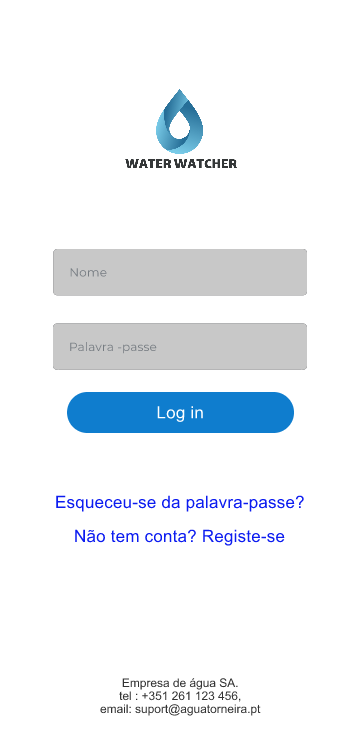
\includegraphics{diagramas/app/1.png}}
\caption{Página de \textit{login}.}
\label{fig:1}
\end{figure}

Nesta página é possível o utilizador inserir as suas credenciais para entrar na aplicação. Também é possível registar uma nova conta ou recuperar o acesso a uma conta. Esta página apresenta também os contactos da empresa.\par
Depois de efetuado o \textit{login}, o utilizador é encaminhado para a página principal, apresentada na Figura \ref{fig:2}.

\begin{figure}[ht!]
\centering
\resizebox{37mm}{!}{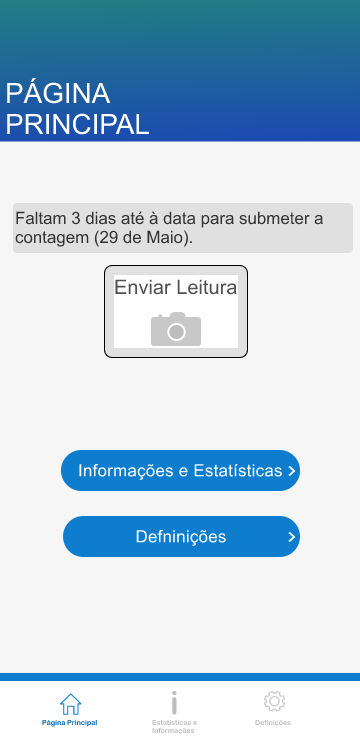
\includegraphics{diagramas/app/2.png}}
\caption{Página principal}
\label{fig:2}
\end{figure}

É neste ecrã que o utilizador poderá enviar a fotografia do contador no dia designado.\par
A partir deste ecrã, tem também a possibilidade de aceder às informações e estatísticas presentes no ecrã representado na Figura \ref{fig:3}. 

%\vspace{8.5cm}

\begin{figure}[ht!]
\centering
\resizebox{40mm}{!}{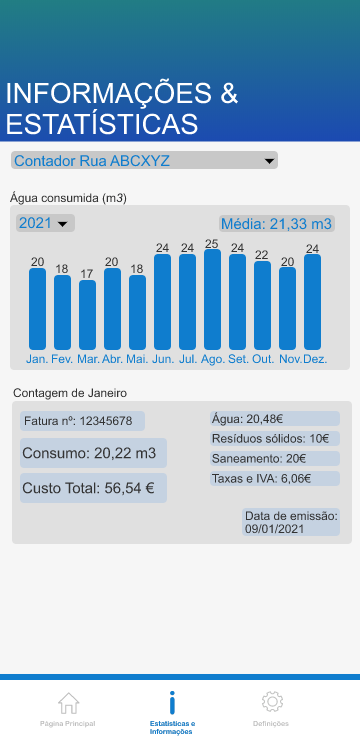
\includegraphics{diagramas/app/3.png}}
\caption{Página de informações e estatísticas}
\label{fig:3}
\end{figure}


A página de informações e estatísticas é onde estão disponíveis vários dados referentes ao serviço e detalhes das faturas do utilizador.\par
Por fim, é possível aceder ao ecrã de definições representado na Figura \ref{fig:4}.

%\vspace{1cm}

\begin{figure}[ht!]
\centering
\begin{minipage}{.5\textwidth}
 \centering
\resizebox{40mm}{!}{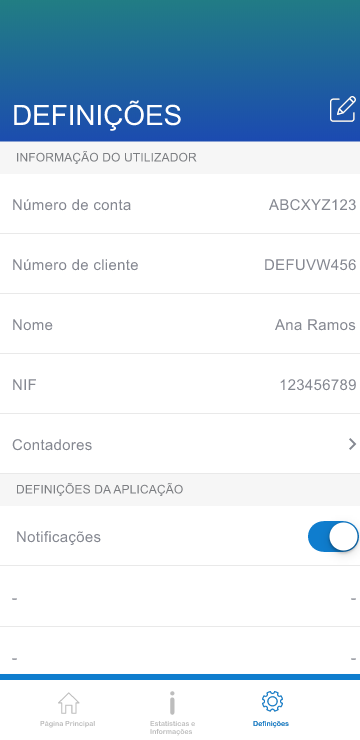
\includegraphics{diagramas/app/4.png}}
\caption{Página de definições.}
\label{fig:4}
\end{minipage}%
\begin{minipage}{.5\textwidth}
  \centering
\resizebox{40mm}{!}{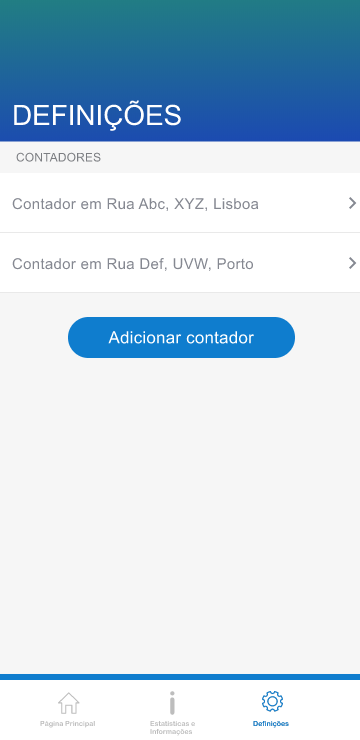
\includegraphics{diagramas/app/5.png}}
\caption{Página de definições relacionadas com os contadores.}
\label{fig:5}
\end{minipage}
\end{figure}

Nesta página, o utilizador pode ver e editar as suas informações e preferências da aplicação. Mais concretamente, também é possível gerir os contadores associados à sua conta, no ecrã da Figura \ref{fig:5}.

\section{Programa de Controlo Semanal} \label{controlo}
Existirá uma forma de os clientes do serviço poderem ter um maior controlo do seu consumo de água, nomeadamente, saber o seu gasto em períodos menores do que mensalmente.\par
Propomos a implementação de um processo, totalmente opcional e que não interfere com a restante utilização do sistema, que lembra os utilizadores semanalmente de enviar a contagem do seu contador.\par
Estes envios terão como propósito poder apresentar ao utilizador o seu gasto de água semanal, permitindo que este, por exemplo, alterando os seus hábitos de consumo de água, consiga observar alterações mais imediatas nas suas contagens. Por outro lado, a empresa prestadora do serviço terá também acesso a estas contagens.\par
Estas contagens têm uma função meramente informativa e são de carater opcional.

%MODELO DE DADOS ......................................................................................
\section{Modelo de Dados} \label{sec:dados}
Um dos componentes deste sistema é um repositório de dados, que irá conter as várias informações relacionadas com os clientes deste serviço. Na Figura \ref{fig:relacoes} está representado de forma gráfica o modelo dos dados guardados neste repositório.\par

\begin{figure}[ht!]
\centering
\resizebox{135mm}{!}{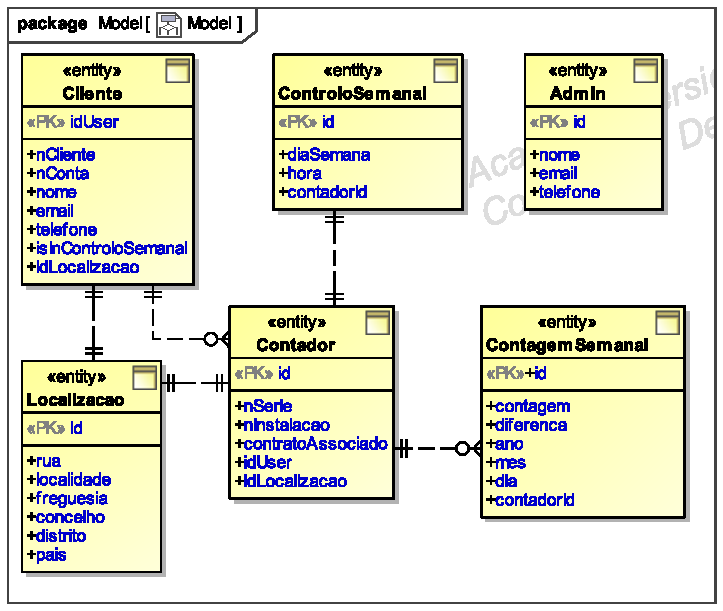
\includegraphics{diagramas/DataModel.pdf}}
\caption{Modelo de dados.}
\label{fig:relacoes}
\end{figure}

A entidade \texttt{Cliente} representa um cliente do serviço que utiliza o sistema. Para cada cliente será registado um ID único \texttt{(IDUser)}, o seu \texttt{nome}, \texttt{email}, número de telefone/telemóvel (\texttt{telefone}), número de cliente (\texttt{nCliente}), número de conta(\texttt{nConta}) e se este cliente está inscrito no controlo semanal (\texttt{isInControloSemanal}).\par
Também existem utilizadores com papel de administrador, representados pela entidade \texttt{Admin} para os quais registamos um ID único (\texttt{id}), o seu \texttt{nome}, \texttt{email} e número de telefone/telemóvel (\texttt{telefone}) .\par
Os clientes terão associado um ou mais contadores, pelo que para cada \texttt{Contador} guardamos um identificador único (\texttt{id}), o seu número de instalação (\texttt{nInstalação}), o seu número de série (\texttt{nSerie}) e o contrato (\texttt{contratoAssociado}) e o cliente (\texttt{iDCliente}) aos quais este contador está associado.\par
Cada contador tem uma \texttt{Localização}, que representa o local onde o contador está instalado. Cada cliente tem também uma localização associada, que representa a sua morada principal para onde é, por exemplo, enviado o correio postal. Uma localização segue a estrutura normal de uma morada: \texttt{rua}, \texttt{localidade}, \texttt{freguesia}, \texttt{concelho}, \texttt{distrito} e \texttt{país}.\par
Existe também uma entidade \texttt{ControloSemanal} que está associada à entidade contador no caso de o cliente a quem pertence este contador estar inscrito no programa de controlo semanal. Essa entidade é composta por um identificador único (\texttt{id}), o contador cujas contagens o cliente vai enviar (\texttt{contadorId}) e o dia da semana e hora que o cliente deseja ser lembrado para efetuar a contagem (\texttt{diaSemana} e \texttt{hora}, respetivamente). \par
Por fim, existe a entidade \texttt{ContagemSemanal} que representa uma contagem semanal submetida pelo cliente, composta por um identificador único (\texttt{id}), pela \texttt{contagem} do contador, pela \texttt{diferença} em relação à contagem do mês anterior, pelo \texttt{ano}, \texttt{mês} e \texttt{dia} em que a contagem foi submetida e pelo identificador do contador associado a esta contagem (\texttt{idContador}).


\section{Reconhecimento de Caracteres} \label{sec:caracteres}
Este sistema vai reconhecer caracteres presentes nas fotografias dos contadores dos clientes. Para melhorar a qualidade e eficácia do reconhecimento de caracteres decidimos estudar e testar vários tipos de imagens de um contador para perceber em quais é que o reconhecimento de caracteres era mais eficaz.
Para este teste utilizamos as seguintes imagens:\\
\par1-Imagem digital de números pretos em fundo branco, de referência.
\par2-Fotografia do contador.
\par3-Fotografia do contador cortada de forma a só conter o mostrador dos números.
\par4-Fotografia 3 em preto e branco.
\par5-Fotografia 3 com as cores invertidas.
\par6-Fotografia 3 com as dimensões aumentadas.\\

Obtivemos mais sucesso, ou seja, o texto obtido através do reconhecimento de caracteres ser mais próximo dos números reais presentes no contador, com a fotografia restringida ao mostrador do contador com as cores invertidas, o que corresponde à situação 5.

\section{Biblioteca de Reconhecimento de Caracteres} \label{bibc}
Para o reconhecimento de caracteres elaborámos uma extensão Outsystems que tem por base a biblioteca Tesseract \cite{tesseract}. A biblioteca Tesseract é uma biblioteca \textit{open source}, ou seja, que pode ser utilizada sem custos monetários, muito utilizada no reconhecimento de caracteres em imagem por ser facilmente configurável consoante a linguagem ou tipo de caracteres que se pretende extrair. Implementa uma rede neuronal para a deteção dos caracteres e utiliza um ficheiro de configuração configurado para detetar dígitos presente em \cite{digits}.

\section{Segurança} \label{seg}
\textit{Cookies} são estruturas que armazenam informação relativa a uma aplicação web no \textit{web browser} do utilizador dessa aplicação.\par
A plataforma Outsystems permite que as aplicações construídas nesta plataforma possam utilizar vários \textit{cookies} gerados automaticamente que conferem ao sistema uma camada de segurança contra possíveis ataques informáticos que possam aceder ou alterar informações de um utilizador \cite{cookies}. Assim, são armazenados no \textit{web browser} do utilizador \textit{cookies} com valores únicos que identificam unicamente um utilizador, de forma a garantir a identidade do utilizador nas comunicações com o elemento servidor.\par
Estes \textit{cookies} devem ser aceites pelos utilizadores da aplicação, caso contrário algumas funções da aplicação não estarão disponíveis, dado que sem elas existiriam problemas de segurança do sistema.\par
Os principais \textit{cookies} gerados são :
\begin{itemize}
\item ServiceCenter : utilizado na funcionalidade de manter a sessão iniciada.
\item ServiceCenter.sid : utilizado para prevenir ataques de \textit{Session Fixation} \cite{sessfix}, ou seja, prevenir que um atacante possa manipular ou obter o ID de sessão de um utilizador, que é utilizado nas comunicações com o servidor.
\item nr2Users : utilizado para definir o ID de utilizador, que é utilizado nas comunicações com o servidor para identificar a que utilizador corresponde o pedido. Evita ataques de \textit{Cross Site Request Forgery} \cite{crsf} na medida que o possível atacante não se conseguiria identificar como a vítima, perante o servidor, sem ter acesso ao conteúdo deste \textit{cookie}. 
\end{itemize}



















